\documentclass[12pt]{paper}\usepackage[]{graphicx}\usepackage[]{color}
%% maxwidth is the original width if it is less than linewidth
%% otherwise use linewidth (to make sure the graphics do not exceed the margin)
\makeatletter
\def\maxwidth{ %
  \ifdim\Gin@nat@width>\linewidth
    \linewidth
  \else
    \Gin@nat@width
  \fi
}
\makeatother

\definecolor{fgcolor}{rgb}{0.345, 0.345, 0.345}
\newcommand{\hlnum}[1]{\textcolor[rgb]{0.686,0.059,0.569}{#1}}%
\newcommand{\hlstr}[1]{\textcolor[rgb]{0.192,0.494,0.8}{#1}}%
\newcommand{\hlcom}[1]{\textcolor[rgb]{0.678,0.584,0.686}{\textit{#1}}}%
\newcommand{\hlopt}[1]{\textcolor[rgb]{0,0,0}{#1}}%
\newcommand{\hlstd}[1]{\textcolor[rgb]{0.345,0.345,0.345}{#1}}%
\newcommand{\hlkwa}[1]{\textcolor[rgb]{0.161,0.373,0.58}{\textbf{#1}}}%
\newcommand{\hlkwb}[1]{\textcolor[rgb]{0.69,0.353,0.396}{#1}}%
\newcommand{\hlkwc}[1]{\textcolor[rgb]{0.333,0.667,0.333}{#1}}%
\newcommand{\hlkwd}[1]{\textcolor[rgb]{0.737,0.353,0.396}{\textbf{#1}}}%

\usepackage{framed}
\makeatletter
\newenvironment{kframe}{%
 \def\at@end@of@kframe{}%
 \ifinner\ifhmode%
  \def\at@end@of@kframe{\end{minipage}}%
  \begin{minipage}{\columnwidth}%
 \fi\fi%
 \def\FrameCommand##1{\hskip\@totalleftmargin \hskip-\fboxsep
 \colorbox{shadecolor}{##1}\hskip-\fboxsep
     % There is no \\@totalrightmargin, so:
     \hskip-\linewidth \hskip-\@totalleftmargin \hskip\columnwidth}%
 \MakeFramed {\advance\hsize-\width
   \@totalleftmargin\z@ \linewidth\hsize
   \@setminipage}}%
 {\par\unskip\endMakeFramed%
 \at@end@of@kframe}
\makeatother

\definecolor{shadecolor}{rgb}{.97, .97, .97}
\definecolor{messagecolor}{rgb}{0, 0, 0}
\definecolor{warningcolor}{rgb}{1, 0, 1}
\definecolor{errorcolor}{rgb}{1, 0, 0}
\newenvironment{knitrout}{}{} % an empty environment to be redefined in TeX

\usepackage{alltt}
\usepackage[top=1in, bottom= 1in, left= 1in, right= 1in]{geometry} 
\usepackage[USenglish]{babel} % set the language; [greek] -> \textgreek{\euro} for sign
\usepackage{multirow} % For tables
\usepackage{graphicx, subfigure} % For graphics
\usepackage{fancyhdr} % Produces fancy headers
\usepackage{setspace} % allows for vsape
\usepackage{natbib} % package to organize literature --> google it!
\usepackage{verbatim} % For including R-code
\usepackage{booktabs} % nicer tables
\usepackage{alltt} % verbatim + highlighting
\usepackage{amsmath} %boldsymbols
\usepackage{lscape} %Querformat
\usepackage{dcolumn} % align at decimal mark
\usepackage{longtable} % split tables over several pages
\usepackage{enumerate} % alter enumerate items (i,ii,iii etc)
\usepackage[colorlinks=true,citecolor=blue,urlcolor=blue]{hyperref}
\usepackage[title,titletoc]{appendix} % appendix functions
\renewcommand\keywordname{Related Commands}
\setlength{\headheight}{15pt}
%\setlength{\footskip}{9.51996pt}
% http://en.wikibooks.org/wiki/LaTeX/Page_Layout for additional info

\author{Patrick Kraft\textsuperscript{1} \and
Christopher Weber\textsuperscript{2} \and
Matthew Lebo\textsuperscript{1}}
\institution{\textsuperscript{1}Stony Brook University \and
\textsuperscript{2}University of Arizona}
\title{The ArfimaMLM Package for R}
\subtitle{Version 1.3\\\footnotesize{(last update \today)}}
\IfFileExists{upquote.sty}{\usepackage{upquote}}{}
\begin{document}

\pagestyle{fancy}

\fancyhead[L]{\footnotesize{ArfimaMLM}}
\fancyhead[R]{\footnotesize{Documentation}}
\fancyfoot[C]{\thepage} %Seitenzahl

\maketitle

\hrule
\begin{abstract}
\texttt{ArfimaMLM} provides functions to facilitate the estimation of Arfima-MLM for repeated cross-sectional data and pooled cross-sectional time series data. The estimation procedure uses double filtering with Arfima methods to account for autocorrelation in longer RCS followed by the use of multilevel modeling (MLM) to estimate both aggregate- and individual-level parameters simultaneously. This documentation provides a brief description of the general approach, as well as an  introduction of possible model specifications. The main function of the package is \texttt{arfimaMLM}, which implements Arfima and multilevel models on a repeated cross-sectional dataset as described by \citet{lebo2015effective}. Furthermore, the function \texttt{arfimaOLS} uses the same initial procedures but estimates a simple linear model instead of the multilevel model. The package also includes \texttt{arfimaPrep}, which prepares a dataset for subsequent analyses according to the Arfima-MLM framework without estimating the final model itself. \texttt{fd} is a wrapper function to estimate the fractional differencing parameter using \texttt{hurstSpec} of the \texttt{fractal}-package as well as procedures provided by the \texttt{fracdiff}-package (via ML, GPH, and Sperio) and to differentiate the series accordingly (mainly for internal use in \texttt{arfimaMLM},\texttt{arfimaOLS}, and \texttt{arfimaPrep}).
\end{abstract}

\begin{keywords}
\texttt{arfimaMLM}, \texttt{arfimaOLS}, \texttt{arfimaPrep}
\end{keywords}
\hrule

\vfill
\newpage
%\doublespacing


\section{Introduction}

\citet{lebo2015effective} presented Arfima-MLM as a new framework for the analysis of repeated cross-sectional (RCS) data. The authors argued that previous methods either fail to account for possible autocorrelation in datasets with many time points, or do not allow for the simultaneous estimation of aggregate- and individual-level parameters. The method suggested by \citet{lebo2015effective} employs double filtering with Arfima methods to remove temporally deterministic components from the variables of interest. After purging potential autocorrelations, a multilevel model (MLM) is used to estimate the parameters for both, the individual as well as the (aggregate) temporal level variables.

The paper presented here describes the \texttt{ArfimaMLM}-package for the statistical software \texttt{R}, which allows for an easy implementation of the procedures described by \citet{lebo2015effective}. The paper proceeds as follows: the first section will briefly summarize the statistical approach presented by \citet{lebo2015effective}. The following section introduces the \texttt{ArfimaMLM}-package, describes the necessary steps for installation, and provides an overview over the general usage of the package. Subsequently, the package will be applied to a simulated dataset.


\section{Arfima-MLM - Overview}

Statistical analyses in political science are often based on data following a repeated cross-sectional designs. Common examples can be found in survey research, such as the National Annenberg Election Study, the American National Election Studies, or Gallup polls, or other types of data such as congressional roll-calls  and Supreme Court cases (see \citealt{lebo2015effective}). Overall, repeated cross-sectional data structures can be characterized by the fact that individual observations are nested within time. However, in contrast to a panel structure, each unit is only included in the dataset at a single point in time. As \citet{lebo2015effective} point out, previous analyses that did not rely on multilevel models usually focused on either the aggregate- or the individual level when analyzing repeated cross-sectional data, which can lead to incorrect standard errors (in the case of pooling) or a significant information loss (in the case of aggregating over time points). Multilevel modeling overcomes this dichotomy between individual and aggregate perspectives since it allows for the estimation of parameters on both levels. However, a simple multilevel model that does not take into account potential deterministic components on the aggregate level might still yield biased or inconsistent results.

The estimation procedure suggested by \citet{lebo2015effective} combines established approaches used to analyze long time series and multilevel modeling in order to account for potential autocorrelations on the aggregate level.

The first step of the Arfima-MLM approach consists of the estimation of fractional differencing parameters for the aggregate-level variables considered in the analyses and differencing the respective series accordingly (see also \citealt{box1996dynamics}), such that
\begin{equation}
\bar{Y}^*_t=(1-L)^d\bar{Y}_t,
\end{equation}
where $\bar{Y}^*_t$ is the stationary series free of autocorrelation, $L$ is a lag operator, $d$ is the fractional differencing parameter, and $\bar{Y}_t$ is the original series of level means of $Y$ at time $t$. Furthermore, the procedure described by \citet{lebo2015effective} includes the estimation of AR and MA parameters as part of the Arfima ($p$,$d$,$q$) model. The fractional differencing and modeling of AR and MA parameters described above is employed for the dependent variable as well as all remaining independent aggregate-level variables included in the analyses (see \citealt{lebo2015effective} for a more detailed discussion of the approach).

In the following step, the individual-level variables are purged from serial correlation on the aggregate level. For the dependent variable, this is done by subtracting the daily deterministic component ($\bar{Y}_t-\bar{Y}^*_t$) from the individual-level values:
\begin{equation}
y_{it}^{**}=y_{it}-(\bar{Y}_t-\bar{Y}^*_t),\label{eq:ydif}
\end{equation}
where $y_{it}^{**}$ consists of the within-time point, as well as the white-noise between-time point variation.

In order to remove potential autocorrelation from independent (individual-level) variables, the within-time point variation is calculated by subtracting the respective level means at time $t$,
\begin{equation}
x_{it}^{**}=x_{it}-\bar{X}_t,\label{eq:xdif}
\end{equation}
where $x_{it}^{**}$ is the within-time point variation of $x_{it}$, $x_{it}$ is the original individual-level variable, and $\bar{X}_t$ is the variable's level mean at time $t$.

After applying this double-filtering procedure to the variables of interest, the multilevel model can be specified. Consider an example with a dependent variable $y_{it}$, an independent variable $x_{it}$ (both of which are filtered according to the procedure outlined above), as well as a aggregate-level variable Z (which does not vary within time-points). The respective model can be described as follows \citep{lebo2015effective}:
\begin{align}
y_{it}^{**}&=\alpha_{1t}+\beta_1 x_{it}^{**} + \epsilon_{1it} \label{eq:model}\\
\alpha_{1t}&=\alpha_{2t}+\beta_2 \bar{X}_{t}^{*} + \gamma Z_t^* + \epsilon_{2t},
\end{align}
where $y_{it}^{**}$ are the double filtered values for $y_{it}$, $x_{it}^{**}$ are the within-time point variations of $x_{it}$, $\bar{X}_{t}^{*}$ is the fractionally differenced series of $\bar{X}_t$, and $Z_t^*$ is the fractionally differenced series of $Z_t$. As described by \citet{lebo2015effective}, equation~\eqref{eq:model} can be further expanded to incorporate time-varying coefficients at the individual level, e.g. by letting the coefficient for $x_{it}^{**}$ vary across time points:
\begin{equation}
y_{it}^{**}=\alpha_{1t}+\beta_t x_{it}^{**} + \epsilon_{1it}
\end{equation}
The following section describes the \texttt{ArfimaMLM}-package which facilitates the estimation based on the procedure outlined above.


\section{Installing the Package}

\texttt{ArfimaMLM} is available on CRAN and can be installed by executing the following command in \texttt{R}:

\begin{knitrout}
\definecolor{shadecolor}{rgb}{0.969, 0.969, 0.969}\color{fgcolor}\begin{kframe}
\begin{alltt}
\hlkwd{install.packages}\hlstd{(}\hlstr{"ArfimaMLM"}\hlstd{)}
\end{alltt}
\end{kframe}
\end{knitrout}



\noindent Alternatively, the latest (development) version of \texttt{ArfimaMLM} can be installed directly from GitHub (using the \texttt{devtools}-Package):

\begin{knitrout}
\definecolor{shadecolor}{rgb}{0.969, 0.969, 0.969}\color{fgcolor}\begin{kframe}
\begin{alltt}
\hlkwd{library}\hlstd{(devtools)}
\hlkwd{install_github}\hlstd{(}\hlstr{"pwkraft/ArfimaMLM"}\hlstd{)}
\end{alltt}
\end{kframe}
\end{knitrout}

\noindent Now the package is installed to the library. In every new session, the package can now be loaded by executing

\begin{knitrout}
\definecolor{shadecolor}{rgb}{0.969, 0.969, 0.969}\color{fgcolor}\begin{kframe}
\begin{alltt}
\hlkwd{library}\hlstd{(ArfimaMLM)}
\end{alltt}
\end{kframe}
\end{knitrout}

At the current version (1.3), the package consists of three major functions: \texttt{arfimaMLM}, \texttt{arfimaOLS}, and \texttt{arfimaPrep}, as well as \texttt{fd}, which is mainly for internal use within the remaining functions.\footnote{For details, execute \texttt{?arfimaMLM}, \texttt{?arfimaOLS}, \texttt{?arfimaPrep}, or \texttt{?fd} in \texttt{R}, or refer to the package manual.} \texttt{arfimaMLM} employs the data manipulations and analyses for a given repeated cross-sectional dataset as specified above. \texttt{ArfimaOLS} performs the same data manipulations but ultimately estimates a linear model instead of a multilevel model. \texttt{arfimaPrep} allows the user to manipulate the data according to the framework specified above, but without estimating a final model. \texttt{fd} is a wrapper function for the \texttt{fracdiff}-package for internal use within \texttt{arfimaPrep}. The following section will provide an introduction for the usage of the \texttt{arfimaMLM} command on the basis of a simulated dataset.


\section{Using the arfimaMLM-command - A Brief Example}

\subsection{Simulating a Repeated Cross-Sectional Dataset}



In order to demonstrate the usage of the \texttt{arfimaMLM} command, we constructed a simulational scenario of a repeated cross-sectional dataset with 100 time points and 500 units within each time point. The dataset contains four different independent variables: $x_1$, $x_2$, $z_1$, and $Z_2$. $x_1$ is normally distributed with mean $\bar{X}_{1t}$ and a standard deviation of 2. Across time points $t$, $\bar{X}_{1t}$ follows a fractionally integrated series with $d=0.3$ and a mean of 5. $x_2$ is normally distributed with a mean of 0 and a standard deviation of 40. The mean of $x_2$ is constant across all time points. $z_1$ is constructed similar to $x_1$: the variable is normally distributed with a mean of $\bar{Z}_{1t}$ and a standard deviation of 3. $\bar{Z}_{1t}$ follows a fractionally integrated series with $d=0.1$ and a mean of 2. $Z_{2t}$ follows a fractionally integrated series with $d=0.25$ and a mean of 3. $Z_{2t}$ does not differ within time points. The dependent variable $y$ is constructed as follows:
\begin{align}
y &=\bar{Y}_t+\beta_{1t} * x_1 - 0.05 * x_2 + 0.3 * \bar{Z}_{1t} + 0 * Z_{2t} + \epsilon &\text{ , where} \nonumber \\
\beta_{1t} &\sim N(0.2,\sigma^2=0.1) & \nonumber \\
\epsilon &\sim N(0,\sigma^2=1), &
\end{align}
where $\bar{Y}_t$ follows a fractionally integrated series with $d=0.4$ and a mean of 10. Note that $\beta_{1t}$ is a random coefficient that varies between time points and that the level variable $Z_{2t}$ actually has \textit{no} effect on $y$. In the dataset, we observe the the following variables: $y$, $x_1$, $x_2$, and $z_1$ for each individual $i$, as well as $Z_{2t}$ for each time point $t$. It is worth noting that in this scenario, it is the aggregate level at time $t$ of $z_1$ that affects $y$, while we measure the variable on an individual level. This aspect was included to demonstrate the possibility of testing aggregate level hypotheses based on individual level data within the \texttt{arfimaMLM} package without prior data manipulations.

The following figures provide an overview over the data simulated for further analyses. Figure~\ref{fig:dv} displays the individual level data points for $y$ as well as the underlying fractionally integrated mean $\bar{Y}_t$.

\begin{figure}[ht]\centering
\caption{Plot of Dependent Variable y Across Time}\label{fig:dv}
\begin{knitrout}
\definecolor{shadecolor}{rgb}{0.969, 0.969, 0.969}\color{fgcolor}
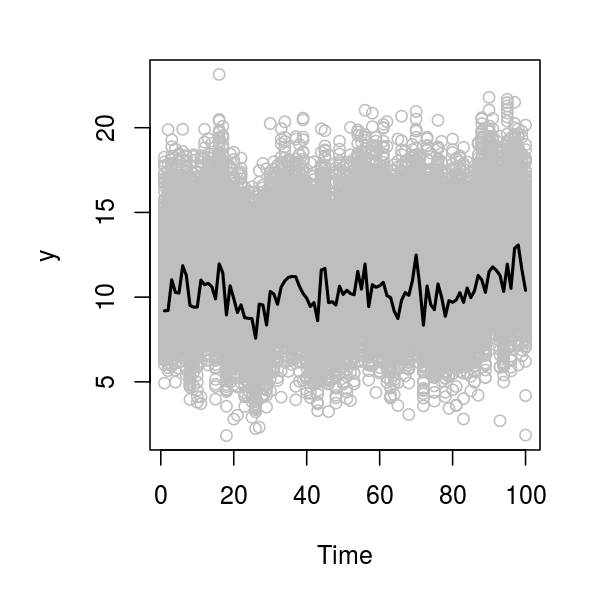
\includegraphics[width=\maxwidth]{figure/unnamed-chunk-6-1} 

\end{knitrout}
\end{figure}

Unsurprisingly, it can be observed that the fractionally integrated structure of the level means manifests itself in the central tendencies of the individual variable values at time $t$. Figure~\ref{fig:ivs} displays the same plots for the four independent variables.

\begin{figure}[ht]\centering
\caption{Plot of Independent Variables Across Time}\label{fig:ivs}
\begin{knitrout}
\definecolor{shadecolor}{rgb}{0.969, 0.969, 0.969}\color{fgcolor}
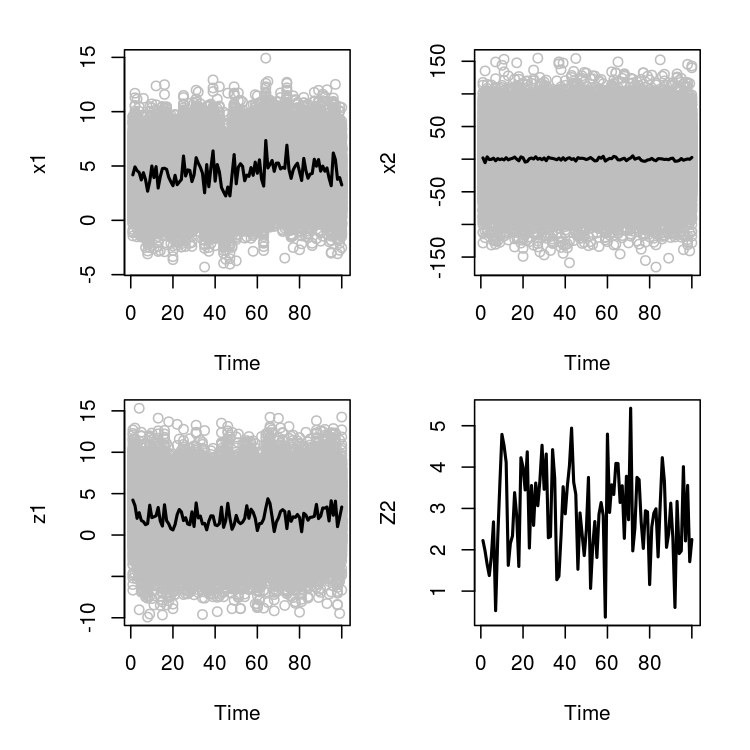
\includegraphics[width=\maxwidth]{figure/unnamed-chunk-7-1} 

\end{knitrout}
\end{figure}

Both individual level variables that were specified to follow an underlying fractionally integrated mean ($x_1$ and $z_1$) show the same pattern as the dependent variable $y$. As specified in the model, the mean of $x_2$ does not vary across time points. For $Z_2$, no individual level variables are observed, so the plot only displays the respective level means at time $t$.

After presenting the simulational scenario, we will now turn to the discussion of the model estimation.

\subsection{Model Estimation}

As already outlined above, the dataset only contains the following variables $x_1$, $x_2$, $z_1$, $Z_2$ and $y$. Calling the head of the data frame in \texttt{R} yields the following output:

\begin{knitrout}
\definecolor{shadecolor}{rgb}{0.969, 0.969, 0.969}\color{fgcolor}\begin{kframe}
\begin{alltt}
\hlkwd{head}\hlstd{(data)}
\end{alltt}
\begin{verbatim}
  time        x1        x2         z1       z2         y
1    1 4.0377894 -32.12057  6.4554502 2.222936 12.250030
2    1 1.8475985 -98.35277  6.5237611 2.222936 15.278788
3    1 2.9154049  33.02954 -1.7316546 2.222936  8.544409
4    1 4.1272183  95.09765  2.3748715 2.222936  6.813665
5    1 5.5262933 -18.80429  6.1095797 2.222936 11.634492
6    1 0.8838083 -10.80839  0.7090984 2.222936 10.483916
\end{verbatim}
\end{kframe}
\end{knitrout}

It is worth noting again that $x_1$, $x_2$, and $y$ are only included as individual-level variables. $z_1$ is also included as an individual-level variable but we are ultimately interested in the estimation of the level effect of $\bar{Z}_t$. $Z_2$ on the other hand does not vary between time points.

In order to be able to compare the model estimates of \texttt{arfimaMLM} to other model specification, we will first present the results of a simple linear regression, as well as a multi-level model (including random effects for \texttt{x1}) based on the simulated data. The results are presented in Table~\ref{tab:ols}.


% Table created by stargazer v.5.2 by Marek Hlavac, Harvard University. E-mail: hlavac at fas.harvard.edu
% Date and time: Wed, Nov 18, 2015 - 05:26:08 PM
% Requires LaTeX packages: dcolumn 
\begin{table}[!htbp] \centering 
  \caption{Results for Simple OLS Model and Multilevel Model} 
  \label{tab:ols} 
\begin{tabular}{@{\extracolsep{5pt}}lD{.}{.}{-3} D{.}{.}{-3} } 
\\[-1.8ex]\hline 
\hline \\[-1.8ex] 
 & \multicolumn{2}{c}{\textit{Dependent variable:}} \\ 
\cline{2-3} 
\\[-1.8ex] & \multicolumn{2}{c}{y} \\ 
\\[-1.8ex] & \multicolumn{1}{c}{\textit{OLS}} & \multicolumn{1}{c}{\textit{linear}} \\ 
 & \multicolumn{1}{c}{\textit{}} & \multicolumn{1}{c}{\textit{mixed-effects}} \\ 
\\[-1.8ex] & \multicolumn{1}{c}{(1)} & \multicolumn{1}{c}{(2)}\\ 
\hline \\[-1.8ex] 
 x1 & 0.200^{***} & 0.207^{***} \\ 
  & (0.003) & (0.011) \\ 
  x2 & -0.050^{***} & -0.050^{***} \\ 
  & (0.0002) & (0.0001) \\ 
  z1 & 0.025^{***} & 0.003^{*} \\ 
  & (0.002) & (0.001) \\ 
  z2 & -0.223^{***} & -0.181^{*} \\ 
  & (0.006) & (0.099) \\ 
  Constant & 11.546^{***} & 11.455^{***} \\ 
  & (0.024) & (0.304) \\ 
 \hline \\[-1.8ex] 
Observations & \multicolumn{1}{c}{50,000} & \multicolumn{1}{c}{50,000} \\ 
\hline 
\hline \\[-1.8ex] 
\textit{Note:}  & \multicolumn{2}{r}{$^{*}$p$<$0.1; $^{**}$p$<$0.05; $^{***}$p$<$0.01} \\ 
\end{tabular} 
\end{table} 


While most of the estimates seem to be reasonably close to the scenario specification, it should be noted that the coefficient for $Z_2$ is highly significant even though it was specified to actually have a null effect. It is very likely that this result arises due to the fact that we did not account for autocorrelations in the series of $Z_2$ or $y$, which potentially induced spurious correlations between both variables. Furthermore, the estimated coefficient for $Z_1$ appears to be much smaller than the true value, albeit still being significant.

How can the model be estimated with the \texttt{arfimaMLM} package? The basic structure of the command can be described as follows:

\begin{knitrout}
\definecolor{shadecolor}{rgb}{0.969, 0.969, 0.969}\color{fgcolor}\begin{kframe}
\begin{alltt}
\hlkwd{arfimaMLM}\hlstd{(formula, data, timevar}
          \hlstd{,} \hlkwc{d} \hlstd{=} \hlstr{"Hurst"}\hlstd{,} \hlkwc{arma} \hlstd{=} \hlkwa{NULL}
          \hlstd{,} \hlkwc{ecmformula} \hlstd{=} \hlkwa{NULL}\hlstd{,} \hlkwc{decm} \hlstd{=} \hlstr{"Hurst"}
          \hlstd{,} \hlkwc{drop} \hlstd{=} \hlnum{5}\hlstd{,} \hlkwc{report.data} \hlstd{=} \hlnum{TRUE}\hlstd{, ...)}
\end{alltt}
\end{kframe}
\end{knitrout}

The major input for the function is \texttt{formula}, which specifies the multilevel model to be estimated after the necessary data transformations according to the Arfima-MLM framework were implemented for the dataset specified in \texttt{data}. It can be specified similar to the model call in standard multilevel models estimated via \texttt{lmer}. The only difference is that the variables specified in \texttt{formula} do not have to be equal to the original variable names included in the data frame. Rather, the user can add specific suffixes to each variable in order to call specific data transformations in the \texttt{arfimaMLM} function. In the current version of the package, three specific suffixes are possible: ``\texttt{.ydif}'', ``\texttt{.xdif}'' and ``\texttt{.fd}''.

If the suffix \texttt{.ydif} is added to the dependent variable (e.g. \texttt{y.ydif} instead of \texttt{y}), the function will remove the daily deterministic component from the individual level variable as specified in equation~\eqref{eq:ydif}, such that it only consists of within-time point, as well as non-temporally autocorrelated between-time point variation. If the suffix \texttt{.xdif} is added to an independent variable (e.g. \texttt{x1.xdif} instead of \texttt{x1}), the variable is simply filtered through the time point averages as specified in equation~\eqref{eq:xdif}.

The suffix \texttt{.fd} allows the user to select variables which are supposed to be transformed to a fractionally differenced level-variable (by aggregating individuals over each time point prior to fractionally differencing the series, \texttt{z1} in our example), or variables which are already included as a level-variable in the original dataset and are just supposed to be fractionally differenced before the multilevel model is estimated (\texttt{z2} in our example). Since the suffixes \texttt{.ydif}, \texttt{.xdif}, and \texttt{.fd} are interpreted by the function as calls for specific data transformation procedures, none of the original variable names in \texttt{data} should include them in order to prevent errors in the estimation procedure.

Consider the following examples for possible \texttt{formula} calls in the \texttt{arfimaMLM} package (omitting the remaining arguments) for the dataset specified above:

\begin{knitrout}
\definecolor{shadecolor}{rgb}{0.969, 0.969, 0.969}\color{fgcolor}\begin{kframe}
\begin{alltt}
\hlkwd{arfimaMLM}\hlstd{(y.ydif} \hlopt{~} \hlstd{x1.xdif} \hlopt{+} \hlstd{x2} \hlopt{+} \hlstd{z1.fd} \hlopt{+} \hlstd{z2.fd}
          \hlopt{+} \hlstd{(}\hlnum{1}\hlopt{|}\hlstd{time)}
          \hlstd{,} \hlkwc{data}\hlstd{=data,} \hlkwc{timevar} \hlstd{=} \hlstr{"time"}\hlstd{, ...)}
\hlkwd{arfimaMLM}\hlstd{(y.ydif} \hlopt{~} \hlstd{x1.xdif} \hlopt{+} \hlstd{x2} \hlopt{+} \hlstd{z1.fd} \hlopt{+} \hlstd{z2.fd}
          \hlopt{+} \hlstd{(}\hlnum{1}\hlopt{+}\hlstd{x1.xdif}\hlopt{|}\hlstd{time)}
          \hlstd{,} \hlkwc{data}\hlstd{=data,} \hlkwc{timevar} \hlstd{=} \hlstr{"time"}\hlstd{, ...)}
\end{alltt}
\end{kframe}
\end{knitrout}

For the simulational scenario, we want to filter the variables \texttt{y} and \texttt{x1}. Accordingly, the suffix \texttt{.ydif} is added to the name of the dependent variable, and the suffix \texttt{.xdif} is added to the name of the independent variable in the data frame \texttt{data}. Furthermore, we want to include the level effects of \texttt{z1} and \texttt{z2}. In order to aggregate \texttt{z1} and fractionally difference \texttt{z1} and \texttt{z2}, we add the suffix \texttt{.fd}. The level variable for these transformations is specified by including the respective variable name \texttt{time} as the argument for \texttt{timevar}. Furthermore, this variable is also specified in \texttt{formula} as the variable according to which the observations are nested in the multilevel model. In the second \texttt{arfimaMLM}, we additionally include a random coefficient for \texttt{x1.xdif}.

We can also add an error correction mechanism to the model. Note that the ecm again does not have to be part of the original dataset but rather is generated within the function. The following two examples show how the error correction mechanism can be specified as part of the \texttt{arfimaMLM} procedure.

\begin{knitrout}
\definecolor{shadecolor}{rgb}{0.969, 0.969, 0.969}\color{fgcolor}\begin{kframe}
\begin{alltt}
\hlkwd{arfimaMLM}\hlstd{(y.ydif} \hlopt{~} \hlstd{x1.xdif} \hlopt{+} \hlstd{x2} \hlopt{+} \hlstd{z1.fd} \hlopt{+} \hlstd{z2.fd} \hlopt{+} \hlstd{ecm}
          \hlopt{+} \hlstd{(}\hlnum{1}\hlopt{|}\hlstd{time)}
          \hlstd{,} \hlkwc{data}\hlstd{=data,} \hlkwc{timevar} \hlstd{=} \hlstr{"time"}
          \hlstd{,} \hlkwc{ecmformula} \hlstd{= y.mean} \hlopt{~} \hlstd{x1.mean, ...)}
\hlkwd{arfimaMLM}\hlstd{(y.ydif} \hlopt{~} \hlstd{x1.xdif} \hlopt{+} \hlstd{x2} \hlopt{+} \hlstd{z1.fd} \hlopt{+} \hlstd{z2.fd} \hlopt{+} \hlstd{ecm}
          \hlopt{+} \hlstd{(}\hlnum{1}\hlopt{+}\hlstd{x1.xdif}\hlopt{|}\hlstd{time)}
          \hlstd{,} \hlkwc{data}\hlstd{=data,} \hlkwc{timevar} \hlstd{=} \hlstr{"time"}
          \hlstd{,} \hlkwc{ecmformula} \hlstd{= y.mean} \hlopt{~} \hlstd{x1.mean, ...)}
\end{alltt}
\end{kframe}
\end{knitrout}

\texttt{ecmformula} contains the specification of the co-integration regression to receive the residuals for the error correction mechanism (\texttt{ecm}) included in \texttt{formula} according to a simple linear regression model specification. Note that the variable names included here cannot be the original variable names, but rather have to be supplemented by the suffix \texttt{.mean}, since the ecm is based on the level/time aggregates at time $t$. Again, the mean is calculated based on the level variable specified in \texttt{timevar}, namely \texttt{time}.

If \texttt{formula} contains \texttt{ecm} as one of the independent variables, and \texttt{ecmformula} is correctly specified, the function will include the lag of the fractionally differenced residuals of the co-integration regression as an error correction mechanism in the multilevel model. The ECM does not have to be estimated prior to calling the function.

The remaining arguments entered in the function specify details about the data manipulation. \texttt{d} calls for a specific estimation method for the fractional differencing parameter in the \texttt{fracdiff}-package or the \texttt{fractal}-package (\texttt{"Hurst"}, \texttt{"ML"}, \texttt{"GPH"}, or \texttt{"Sperio"}). The default is \texttt{"Hurst"}. If the user wants to specify the methods for each variable individually, \texttt{d} can be a list containing a call for every individual variable. Furthermore, the list can contain numeric values for differencing parameters which were estimated externally (see example). A variable will not be differenced if \texttt{d} is specified as 0. Accordingly, \texttt{decm} calls for a specific estimation method for the fractional differencing parameter. Again, it can be either \texttt{"Hurst"}, \texttt{"ML"}, \texttt{"GPH"}, or \texttt{"Sperio"} and the default is \texttt{"Hurst"}. Again, the argument can also be a numeric value indicating the differencing parameter estimated externally.

It is also possible to estimate AR and MA parameters for the (fractionally differenced) level variables in order to remove remaining autocorrelation. \texttt{arma} contains a list of variables for which AR and MA parameters are to be estimated (after fractional differencing) as well as a vector containing the respective orders of the model to fit. \texttt{order[1]} corresponds to the AR part and \texttt{order[2]} to the MA part, similar to the model specification in \texttt{arima} (just excluding the d parameter here). For variables specified in \texttt{arma}, the function will use the residuals of the ARMA model (which is estimated for the fractionally differenced level variables, respectively) for the subsequent model estimation in order to remove their deterministic components. This procedure is only available for variables which were augmented by the suffix \texttt{.fd} or \texttt{.ydif} in \texttt{formula}. It is also possible to fix certain AR or MA parameters at zero instead of estimating all parameters up to the order described in \texttt{arma}. For example, one might want to estimate AR(1) and AR(3) parameters, but not include AR(2) for a specific variable in the model.

Consider the following examples for different model specifications taking into account the estimation method for the fractional differencing parameter as well as the estimation of respective ARMA models.

\begin{knitrout}
\definecolor{shadecolor}{rgb}{0.969, 0.969, 0.969}\color{fgcolor}\begin{kframe}
\begin{alltt}
\hlkwd{arfimaMLM}\hlstd{(y.ydif} \hlopt{~} \hlstd{x1.xdif} \hlopt{+} \hlstd{x2} \hlopt{+} \hlstd{z1.fd} \hlopt{+} \hlstd{z2.fd} \hlopt{+} \hlstd{ecm}
          \hlopt{+} \hlstd{(}\hlnum{1}\hlopt{|}\hlstd{time)}
          \hlstd{,} \hlkwc{data}\hlstd{=data,} \hlkwc{timevar} \hlstd{=} \hlstr{"time"}
          \hlstd{,} \hlkwc{ecmformula} \hlstd{= y.mean} \hlopt{~} \hlstd{x1.mean}
          \hlstd{,} \hlkwc{d}\hlstd{=}\hlstr{"Sperio"}
          \hlstd{,} \hlkwc{decm}\hlstd{=}\hlstr{"ML"}\hlstd{, ...)}
\hlkwd{arfimaMLM}\hlstd{(y.ydif} \hlopt{~} \hlstd{x1.xdif} \hlopt{+} \hlstd{x2} \hlopt{+} \hlstd{z1.fd} \hlopt{+} \hlstd{z2.fd} \hlopt{+} \hlstd{ecm}
          \hlopt{+} \hlstd{(}\hlnum{1}\hlopt{+}\hlstd{x1.xdif}\hlopt{|}\hlstd{time)}
          \hlstd{,} \hlkwc{data}\hlstd{=data,} \hlkwc{timevar} \hlstd{=} \hlstr{"time"}
          \hlstd{,} \hlkwc{ecmformula} \hlstd{= y.mean} \hlopt{~} \hlstd{x1.mean}
          \hlstd{,} \hlkwc{d}\hlstd{=}\hlkwd{list}\hlstd{(}\hlkwc{y}\hlstd{=}\hlstr{"Hurst"}\hlstd{,} \hlkwc{z1}\hlstd{=}\hlstr{"Sperio"}\hlstd{,} \hlkwc{z2}\hlstd{=}\hlnum{0.25}\hlstd{)}
          \hlstd{,} \hlkwc{decm}\hlstd{=}\hlstr{"GPH"}\hlstd{, ...)}
\hlkwd{arfimaMLM}\hlstd{(y.ydif} \hlopt{~} \hlstd{x1.xdif} \hlopt{+} \hlstd{x2} \hlopt{+} \hlstd{z1.fd} \hlopt{+} \hlstd{z2.fd} \hlopt{+} \hlstd{ecm}
          \hlopt{+} \hlstd{(}\hlnum{1}\hlopt{+}\hlstd{x1.xdif}\hlopt{|}\hlstd{time)}
          \hlstd{,} \hlkwc{data}\hlstd{=data,} \hlkwc{timevar} \hlstd{=} \hlstr{"time"}
          \hlstd{,} \hlkwc{ecmformula} \hlstd{= y.mean} \hlopt{~} \hlstd{x1.mean}
          \hlstd{,} \hlkwc{arma} \hlstd{=} \hlkwd{list}\hlstd{(}\hlkwc{y} \hlstd{=} \hlkwd{c}\hlstd{(}\hlnum{1}\hlstd{,}\hlnum{0}\hlstd{),} \hlkwc{z2} \hlstd{=} \hlkwd{c}\hlstd{(}\hlnum{0}\hlstd{,}\hlnum{2}\hlstd{)), ...)}
\hlkwd{arfimaMLM}\hlstd{(y.ydif} \hlopt{~} \hlstd{x1.xdif} \hlopt{+} \hlstd{x2} \hlopt{+} \hlstd{z1.fd} \hlopt{+} \hlstd{z2.fd} \hlopt{+} \hlstd{ecm}
          \hlopt{+} \hlstd{(}\hlnum{1}\hlopt{+}\hlstd{x1.xdif}\hlopt{|}\hlstd{time)}
          \hlstd{,} \hlkwc{data}\hlstd{=data,} \hlkwc{timevar} \hlstd{=} \hlstr{"time"}
          \hlstd{,} \hlkwc{ecmformula} \hlstd{= y.mean} \hlopt{~} \hlstd{x1.mean}
          \hlstd{,} \hlkwc{arma} \hlstd{=} \hlkwd{list}\hlstd{(}\hlkwc{y} \hlstd{=} \hlkwd{list}\hlstd{(}\hlnum{1}\hlstd{,}\hlkwd{c}\hlstd{(}\hlnum{1}\hlstd{,}\hlnum{3}\hlstd{))}
                        \hlstd{,} \hlkwc{z2} \hlstd{=} \hlkwd{c}\hlstd{(}\hlnum{0}\hlstd{,}\hlnum{1}\hlstd{)))}
\end{alltt}
\end{kframe}
\end{knitrout}

The first example calls the estimation method \texttt{Sperio} for all respective variables included in \texttt{formula}, and \texttt{ML} for fractionally differencing the error correction mechanism. In the second example, \texttt{d} contains a list specifying the estimation method for each variable individually. Accordingly, \texttt{y} is estimated via \texttt{Hurst}, and \texttt{z1} via \texttt{Sperio}. For \texttt{z2}, the fractional differencing parameter was externally set to $0.25$. The fractional integration parameter for the error correction mechanism is estimated via \texttt{GPH}. While it is unlikely that such a detailed specification of estimation mechanisms is necessary (or useful), this example was merely supposed to demonstrate the flexibility of the function. In the third example, the estimation of the d parameters for all respective variables in \texttt{formula} and \texttt{ecm} is kept at the default (\texttt{Hurst}). However, additionally to fractional differencing, the function also estimates an AR(1) model for \texttt{y} and a MA(2) model for \texttt{z2}. Note that the MA(2) model will provide estimates for both, MA(1) and MA(2). The multilevel model estimated subsequently would include the residuals of the AR/MA model estimated after fractionally differencing the respective variables. The last example presents a more complex ARMA model specification for \texttt{y} than in the previous example. The only difference is, that the argument indicating the order of the ARMA model for \texttt{y} is a list (\texttt{list(1,c(1,3))}) instead of a vector (\texttt{c(1,0)}). This implies that the ARMA model does not include all parameters up to the highest order specified (as in the previous example), but rather only include the AR and MA parameters that are explicitly listed. Again, the first element corresponds to the AR part, while the second element corresponds to the MA part of the model. Accordingly, \texttt{arma = list(y = list(1,c(1,3)))} will estimate AR(1), MA(1) and MA(3) parameters for y, while \texttt{arma = list(y = c(1,3))} would yield estimates for AR(1), MA(1), MA(2), as well as MA(3).

The last two arguments that can be specified are \texttt{drop}, which determines the number of initial time points to be dropped from the analysis (default is 5), as well as \texttt{report.data}, which determines whether the model output should include the transformed dataset used for the analysis (default is \texttt{TRUE}). Furthermore, additional arguments can be passed to the estimation procedures used within the function (e.g. for \texttt{lmer}).

After describing the details about the model specification, we will now turn to a brief discussion of the function's output. In general, the function returns a list of the S3 class \texttt{`arfimaMLM'} with the following items:
\begin{itemize}
\item \texttt{result}: Output of the multilevel model as specified in \texttt{formula}.
\item \texttt{ecm}: Output of the co-integration regression (returned if \texttt{ecmformula} is specified). The lagged residuals of the co-integration regression are included in the multilevel model if \texttt{ecm} is included in \texttt{formula}.
\item \texttt{d}: Matrix of fractional differencing parameters estimated for the level variables (\texttt{.ydif} and \texttt{.fd}) as well as the estimation method for each variable. Returns the specified value for d if it was specified in the initial call of the function.
\item \texttt{arma}: List of \texttt{arima} results for each variable specified in the model call. Contains AR/MA estimates as well as the model residuals.
\item \texttt{data.mean}: Data frame of variable means declared in \texttt{formula} as \texttt{.ydif}, \texttt{.xdif} or \texttt{.fd} for each time point specified by the level variable in \texttt{formula}.
\item \texttt{data.fd}: Data frame of fractionally differenced level variables declared in \texttt{formula} as \texttt{.ydif} or \texttt{.fd} for each time point specified by the level variable in \texttt{formula}.
\item \texttt{data.merged}: Merged data frame used when estimating the multilevel model consisting of the original data as well as \texttt{data.mean} and \texttt{data.fd}
\end{itemize}

Note that \texttt{data.mean}, \texttt{data.fd}, and \texttt{data.merged} are only included if \texttt{report.data} is set at its default (i.e. \texttt{TRUE}). Consider the following example for the simulational scenario specified in this paper:

\begin{knitrout}
\definecolor{shadecolor}{rgb}{0.969, 0.969, 0.969}\color{fgcolor}\begin{kframe}
\begin{alltt}
\hlstd{m1} \hlkwb{<-} \hlkwd{arfimaMLM}\hlstd{(y.ydif} \hlopt{~} \hlstd{x1.xdif} \hlopt{+} \hlstd{x2} \hlopt{+} \hlstd{z1.fd} \hlopt{+} \hlstd{z2.fd}
                \hlopt{+} \hlstd{ecm} \hlopt{+} \hlstd{(}\hlnum{1}\hlopt{+}\hlstd{x1.xdif}\hlopt{|}\hlstd{time)}
                \hlstd{,} \hlkwc{data} \hlstd{= data,} \hlkwc{timevar} \hlstd{=} \hlstr{"time"}
                \hlstd{,} \hlkwc{ecmformula} \hlstd{= y.mean} \hlopt{~} \hlstd{x1.mean}
                \hlstd{,} \hlkwc{d} \hlstd{=} \hlstr{"Hurst"}
                \hlstd{,} \hlkwc{decm} \hlstd{=} \hlstr{"GPH"}\hlstd{)}
\end{alltt}
\end{kframe}
\end{knitrout}

Calling the summary of this model will provide a brief \texttt{R}-Output that summarizes the most important results:

\begin{knitrout}
\definecolor{shadecolor}{rgb}{0.969, 0.969, 0.969}\color{fgcolor}\begin{kframe}
\begin{alltt}
\hlkwd{summary}\hlstd{(m1)}
\end{alltt}
\begin{verbatim}

###################################
Summary Error Correction Mechanism: 

Call:
lm(formula = ecmformula, data = data.mean)

Residuals:
    Min      1Q  Median      3Q     Max 
-3.2427 -0.7130  0.0182  0.7618  2.6427 

Coefficients:
            Estimate Std. Error t value Pr(>|t|)    
(Intercept)  11.1164     0.5400  20.584   <2e-16 ***
x1.mean       0.1630     0.1194   1.364    0.176    
---
Signif. codes:  0 '***' 0.001 '**' 0.01 '*' 0.05 '.' 0.1 ' ' 1

Residual standard error: 1.13 on 98 degrees of freedom
Multiple R-squared:  0.01864,	Adjusted R-squared:  0.008626 
F-statistic: 1.861 on 1 and 98 DF,  p-value: 0.1756


###################################
Fractional Differencing Parameters: 

    Method   Estimate
y    Hurst 0.41713434
z1   Hurst 0.01679005
z2   Hurst 0.10887414
ecm    GPH 0.55248930


#########################
Summary Multilevel Model: 

Linear mixed model fit by REML ['lmerMod']
Formula: y.ydif ~ x1.xdif + x2 + z1.fd + z2.fd + ecm + (1 + x1.xdif |  
    time)
   Data: new$data.merged

REML criterion at convergence: 136183.4

Scaled residuals: 
    Min      1Q  Median      3Q     Max 
-4.2365 -0.6678  0.0050  0.6697  4.0721 

Random effects:
 Groups   Name        Variance Std.Dev. Corr
 time     (Intercept) 1.11753  1.057        
          x1.xdif     0.01167  0.108    0.47
 Residual             1.01005  1.005        
Number of obs: 47500, groups:  time, 95

Fixed effects:
              Estimate Std. Error t value
(Intercept)  0.0600844  0.1087158     0.6
x1.xdif      0.2035655  0.0113217    18.0
x2          -0.0499160  0.0001156  -431.7
z1.fd        0.2360076  0.1037031     2.3
z2.fd       -0.0468624  0.0943287    -0.5
ecm         -0.1497914  0.0873453    -1.7

Correlation of Fixed Effects:
        (Intr) x1.xdf x2     z1.fd  z2.fd 
x1.xdif  0.455                            
x2       0.000  0.000                     
z1.fd    0.030  0.000  0.000              
z2.fd   -0.036  0.000 -0.001  0.005       
ecm     -0.030  0.000  0.000 -0.021  0.077
\end{verbatim}
\end{kframe}
\end{knitrout}

Looking at the coefficients estimated in the multilevel model of the \texttt{arfimaMLM} function, it can be seen that the coefficients are closer to the values specified in the simulational scenario as compared to the estimates reported for the simple OLS model (see Table~\ref{tab:ols}). More specifically, the estimate for \texttt{z1} is closer to its true value. More importantly, taking into account the time-series structure of the level-variables eliminates the significant effect of \texttt{z2}. While this evidence by itself is obviously not sufficient to show that the ArfimaMLM procedure yields more consistent estimates in general, it certainly provides additional evidence in favor of the findings presented by \citet{lebo2015effective}.

We can also extract specific items from the \texttt{arfimaMLM}-list. Let's assume we were only interested in the result of the multilevel model. Furthermore, we would like to take a look at the head of the fractionally differenced data as well as the data containing the generated means for each time point. We would also like to save the merged data frame used for the analysis for future use. All of that can be implemented by executing the following code:

\begin{knitrout}
\definecolor{shadecolor}{rgb}{0.969, 0.969, 0.969}\color{fgcolor}\begin{kframe}
\begin{alltt}
\hlkwd{summary}\hlstd{(m1}\hlopt{$}\hlstd{result)}
\end{alltt}
\begin{verbatim}
Linear mixed model fit by REML ['lmerMod']
Formula: y.ydif ~ x1.xdif + x2 + z1.fd + z2.fd + ecm + (1 + x1.xdif |  
    time)
   Data: new$data.merged

REML criterion at convergence: 136183.4

Scaled residuals: 
    Min      1Q  Median      3Q     Max 
-4.2365 -0.6678  0.0050  0.6697  4.0721 

Random effects:
 Groups   Name        Variance Std.Dev. Corr
 time     (Intercept) 1.11753  1.057        
          x1.xdif     0.01167  0.108    0.47
 Residual             1.01005  1.005        
Number of obs: 47500, groups:  time, 95

Fixed effects:
              Estimate Std. Error t value
(Intercept)  0.0600844  0.1087158     0.6
x1.xdif      0.2035655  0.0113217    18.0
x2          -0.0499160  0.0001156  -431.7
z1.fd        0.2360076  0.1037031     2.3
z2.fd       -0.0468624  0.0943287    -0.5
ecm         -0.1497914  0.0873453    -1.7

Correlation of Fixed Effects:
        (Intr) x1.xdf x2     z1.fd  z2.fd 
x1.xdif  0.455                            
x2       0.000  0.000                     
z1.fd    0.030  0.000  0.000              
z2.fd   -0.036  0.000 -0.001  0.005       
ecm     -0.030  0.000  0.000 -0.021  0.077
\end{verbatim}
\begin{alltt}
\hlkwd{head}\hlstd{(m1}\hlopt{$}\hlstd{data.fd)}
\end{alltt}
\begin{verbatim}
  time       y.fd      z1.fd       z2.fd        ecm
1    1 -0.4980316  1.9757137 -0.65226663         NA
2    2  0.4986830  1.3185836 -0.83418872 -0.4669326
3    3  0.7585310 -0.1471850 -1.10178838  0.4668722
4    4 -0.1486040  0.3205121 -1.30089067  0.7160995
5    5 -0.2049091 -0.2496606 -0.75823137 -0.2124583
6    6  0.3718751 -0.5550096  0.05193581 -0.1185358
\end{verbatim}
\begin{alltt}
\hlkwd{head}\hlstd{(m1}\hlopt{$}\hlstd{data.mean)}
\end{alltt}
\begin{verbatim}
  time   y.mean  x1.mean  z1.mean  z2.mean
1    1 11.33888 4.230249 4.154311 2.222936
2    2 12.12785 4.924501 3.530353 1.969999
3    3 12.65626 4.700633 2.070416 1.643219
4    4 12.03351 4.320279 2.519231 1.376323
5    5 11.81165 3.712363 1.949179 1.851921
6    6 12.27197 4.375128 1.633863 2.674118
\end{verbatim}
\begin{alltt}
\hlstd{newdata} \hlkwb{<-} \hlstd{m1}\hlopt{$}\hlstd{data.merged}
\end{alltt}
\end{kframe}
\end{knitrout}

The same model can also be estimated using \texttt{arfimaOLS}. All arguments with regard to the data manipulations and model specification are equivalent to \texttt{arfimaMLM}. The only difference is that \texttt{arfimaOLS} ultimately estimates a simple linear regression model rather than a multilevel model. Consider the following specification of the same model using \texttt{arfimaOLS}:

\begin{knitrout}
\definecolor{shadecolor}{rgb}{0.969, 0.969, 0.969}\color{fgcolor}\begin{kframe}
\begin{alltt}
\hlstd{m2} \hlkwb{<-} \hlkwd{arfimaOLS}\hlstd{(y.ydif} \hlopt{~} \hlstd{x1.xdif} \hlopt{+} \hlstd{x2} \hlopt{+} \hlstd{z1.fd} \hlopt{+} \hlstd{z2.fd}
                \hlopt{+} \hlstd{ecm}
                \hlstd{,} \hlkwc{data} \hlstd{= data,} \hlkwc{timevar} \hlstd{=} \hlstr{"time"}
                \hlstd{,} \hlkwc{ecmformula} \hlstd{= y.mean} \hlopt{~} \hlstd{x1.mean}
                \hlstd{,} \hlkwc{d} \hlstd{=} \hlstr{"Hurst"}
                \hlstd{,} \hlkwc{decm} \hlstd{=} \hlstr{"GPH"}\hlstd{)}
\end{alltt}
\end{kframe}
\end{knitrout}

The only difference in the function call for \texttt{arfimaOLS} is the fact that \texttt{formula} does not include the specification for clustering. All other arguments, function calls, as well as the structure of the output is equivalent to the description outlined above.\footnote{It should be noted that the S3 class of this model output is \texttt{arfimaOLS} and not \texttt{arfimaMLM}. However, both classes are essentially equivalent with regard to their structure and behavior.} Again, calling the summary of this model will provide a brief \texttt{R}-Output that summarizes the most important results:

\begin{knitrout}
\definecolor{shadecolor}{rgb}{0.969, 0.969, 0.969}\color{fgcolor}\begin{kframe}
\begin{alltt}
\hlkwd{summary}\hlstd{(m2)}
\end{alltt}
\begin{verbatim}

###################################
Summary Error Correction Mechanism: 

Call:
lm(formula = ecmformula, data = data.mean)

Residuals:
    Min      1Q  Median      3Q     Max 
-3.2427 -0.7130  0.0182  0.7618  2.6427 

Coefficients:
            Estimate Std. Error t value Pr(>|t|)    
(Intercept)  11.1164     0.5400  20.584   <2e-16 ***
x1.mean       0.1630     0.1194   1.364    0.176    
---
Signif. codes:  0 '***' 0.001 '**' 0.01 '*' 0.05 '.' 0.1 ' ' 1

Residual standard error: 1.13 on 98 degrees of freedom
Multiple R-squared:  0.01864,	Adjusted R-squared:  0.008626 
F-statistic: 1.861 on 1 and 98 DF,  p-value: 0.1756


###################################
Fractional Differencing Parameters: 

    Method   Estimate
y    Hurst 0.41713434
z1   Hurst 0.01679005
z2   Hurst 0.10887414
ecm    GPH 0.55248930


##################
Summary OLS Model: 

Call:
lm(formula = formula, data = new$data.merged)

Residuals:
    Min      1Q  Median      3Q     Max 
-6.0890 -0.9588  0.0402  1.0017  5.7285 

Coefficients:
              Estimate Std. Error  t value Pr(>|t|)    
(Intercept)  0.0613607  0.0067106    9.144   <2e-16 ***
x1.xdif      0.2033355  0.0033485   60.724   <2e-16 ***
x2          -0.0499045  0.0001677 -297.662   <2e-16 ***
z1.fd        0.2076489  0.0071888   28.885   <2e-16 ***
z2.fd       -0.0846972  0.0065389  -12.953   <2e-16 ***
ecm         -0.1696242  0.0060560  -28.009   <2e-16 ***
---
Signif. codes:  0 '***' 0.001 '**' 0.01 '*' 0.05 '.' 0.1 ' ' 1

Residual standard error: 1.46 on 47494 degrees of freedom
Multiple R-squared:  0.6641,	Adjusted R-squared:  0.664 
F-statistic: 1.878e+04 on 5 and 47494 DF,  p-value: < 2.2e-16
\end{verbatim}
\end{kframe}
\end{knitrout}

Again, the estimate for \texttt{z1} appears to be closer to its true value as compared to the original OLS results. However, since we did not properly take into account the multilevel structure as in \texttt{arfimaMLM}, the coefficient for \texttt{z2} still remains significant (albeit being closer to zero than the coefficient reported in Table~\ref{tab:ols}).

\bibliographystyle{/data/Copy/1-src/lit/apsr}
\bibliography{/data/Copy/1-src/lit/Literature}
\end{document}
